\documentclass[11pt,a4paper]{article}
\usepackage[hyperref]{emnlp2018}
\usepackage{times}
\usepackage{url}
\usepackage{amsmath,amsfonts,amssymb}
\usepackage{paralist}
\usepackage{color,xcolor}
\usepackage{bm}
\usepackage{multirow}
\usepackage{makecell}
\usepackage{caption}
\usepackage[linesnumbered,lined]{algorithm2e}
\usepackage{todonotes}

% bold x for equations
\newcommand{\rmx}{\mathrm x} 
% used for table headers
\newcommand{\tabh}[1]{\multicolumn{1}{c|}{\textbf{#1}}}  
% used for the top left cell in a table
\newcommand{\tabc}[2]{\multicolumn{1}{|c|}{\multirow{#1}{*}{\textbf{#2}}}} 
% used for denoting the loss symbol with a subscript
\newcommand{\loss}[1]{J_\text{#1}}

%\aclfinalcopy % Un-comment this line for the final submission
%\def\aclpaperid{***} %  Enter the acl Paper ID here

%\setlength\titlebox{5cm}
% You can expand the titlebox if you need extra space
% to show all the authors. Please do not make the titlebox
% smaller than 5cm (the original size); we will check this
% in the camera-ready version and ask you to change it back.
\title{Disentangled Representation Learning for Linguistic Style Transfer}

\author{First Author \\
  Affiliation / Address line 1 \\
  {\tt email@domain} \\\And
  Second Author \\
  Affiliation / Address line 1 \\
  {\tt email@domain} \\}

\date{}

\begin{document}

\maketitle

\graphicspath{{images/}}


\begin{abstract}
	This paper tackles the problem of disentangling the style and content latent spaces of language models. We propose a simple yet effective approach, which incorporates auxiliary objectives: a multi-task classification objective, and dual adversarial objectives for label prediction and bag-of-words prediction, respectively. We show, both qualitatively and quantitatively, that the style and content are indeed disentangled in the latent space, using this approach. We apply this disentangled latent representation learning method to attribute / label / style transfer in natural language generation. We achieve similar content preservation scores compared to previous state-of-the-art approaches, and significantly better style-transfer strength scores. Our code is made publicly available for reproduction and extension purposes~\footnote{\url{https://github.com/vineetjohn/linguistic-style-transfer}}.
\end{abstract}

% 


\section{Introduction}

The neural network has been a successful learning machine during the past decade due to its highly expressive modeling capability, which is a consequence of multiple layers of non-linear transformation of input features. Such transformations, however, make intermediate features `latent', in that they do not have explicit meaning and are not explainable. Therefore, neural networks are usually treated as black-box machinery.

Disentangling the latent space of neural networks has become an increasingly important research topic. In the image domain, for example, \citet{chen2016infogan} use adversarial and information maximization objectives to produce interpretable latent representations that can be tweaked to adjust writing style for handwritten digits, as well as lighting and orientation for face models. \citet{mathieu2016disentangling} utilize a convolutional autoencoder to achieve the same objective. However, this problem is not well explored in natural language processing.

In this paper, we address the problem of disentangling the latent space of neural networks' for text generation. Our model is built on an autoencoder that learns the latent space (vector representation) of a sentence by decoding the sentence itself. We would like the latent space to be disentangled with respect to different features, namely, \textit{style} and \textit{content}.

To accomplish this, we propose a simple approach that combines multi-task and adversarial objectives. We artificially divide the latent representation into two parts: style space and content space. We learn model parameters that produce separate style and content latent spaces from the encoded sentence representation. The multi-task objective operates on the style space to ensure it does contain style information. The adversarial style objective, on the contrary, operates on the content space to minimize the predictability of style. In addition, the bag-of-words adversary minimizes the predictability of original words of the sentence in the style space. In this way, the style and content variables can be disentangled from each other.

These representation learning objectives can be directly used for style transfer in sentence generation~\cite{hu2017toward,shen2017style,fu2017style}, in which a model can generate a sentence with the same content, but a different style. We simply use an autoencoder to encode the content vector of a sentence, but ignore its encoded style vector. Then we infer from the training data, an empirical embedding of the style that we want to transfer. The encoded content vector and the inferred style vector are concatenated and fed to the autoencoder for decoding. Using this grafting technique, we generate a new sentence similar in content but different in style.

We conducted experiments on two customer review benchmark datasets. Both qualitative and quantitative results show that the style vector does contain most style information, whereas the content vector contains little (if any). In the empirical style-transfer evaluations, we achieve significantly better style transfer scores than previous results, while obtaining better or comparable content preservation scores. We also show, using ablation tests, that the auxiliary losses can be combined well, each playing its own role in disentangling the latent space.


\begin{figure}[ht]
	\centering
	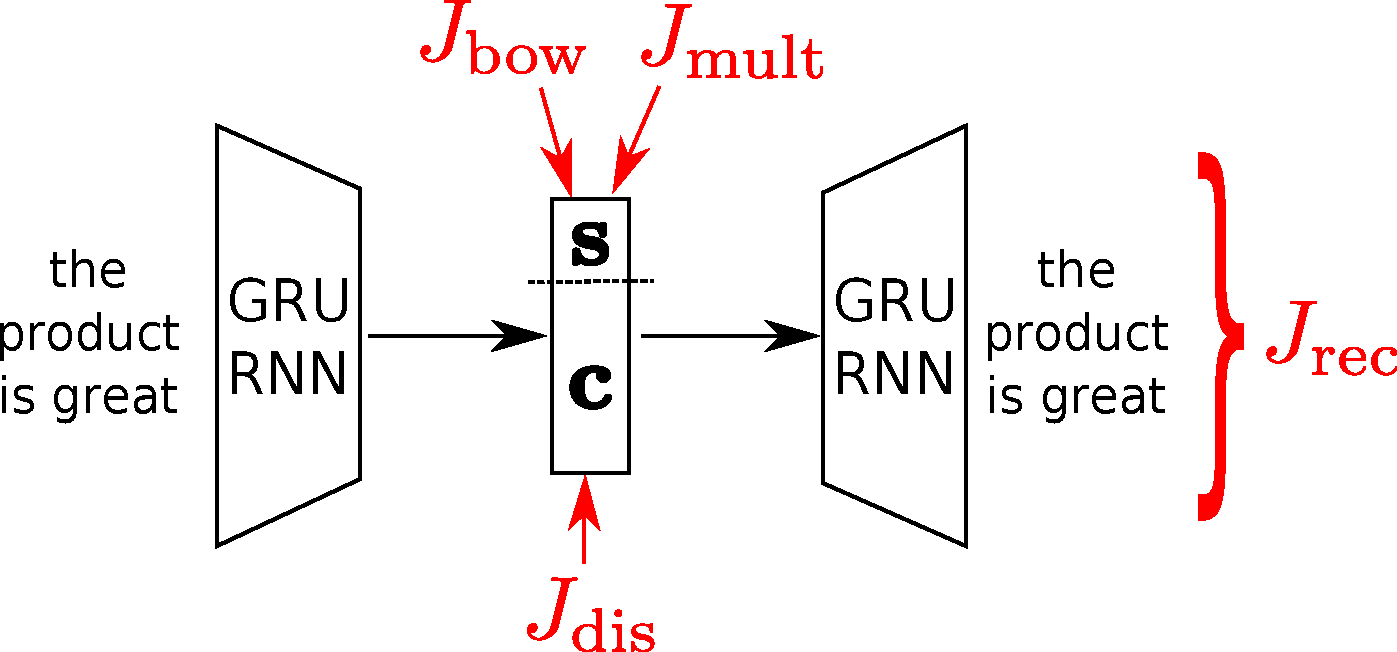
\includegraphics[width=0.8\linewidth]{model-overview-training}
	\caption{Model Training Overview}
	\label{fig:model-training-overview}
\end{figure}
\begin{figure}[ht]
	\centering
	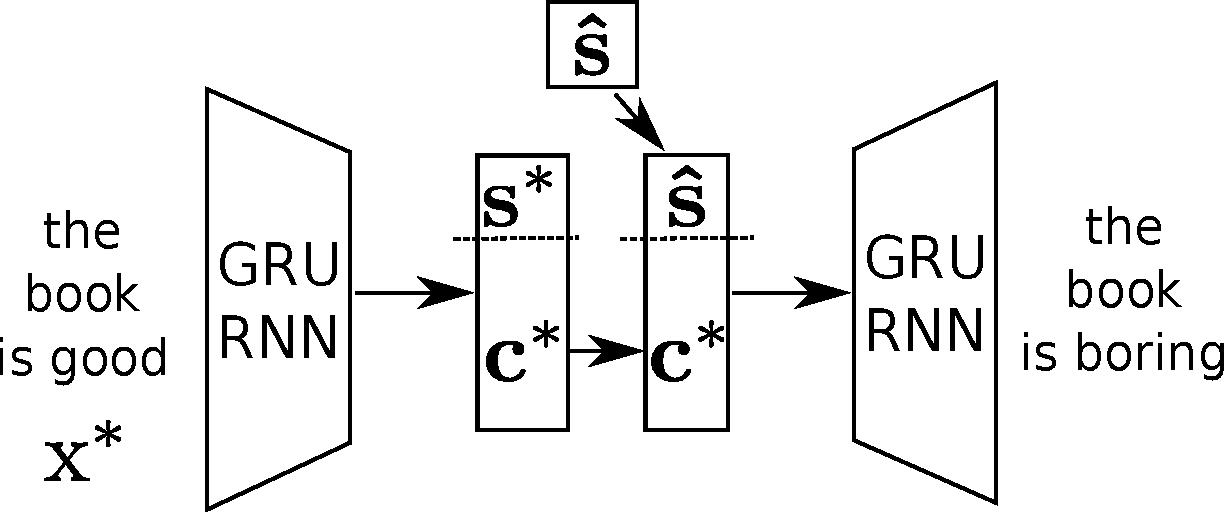
\includegraphics[width=0.8\linewidth]{model-overview-inference}
	\caption{Model Generation Overview}
	\label{fig:model-inference-overview}
\end{figure}



\section{Related Work}

Disentangling latent space has been explored in the image processing domain in the recent years, and researchers have successfully disentangled rotation features, color features, etc.~\cite{chen2016infogan,luan2017deep}. Some image styles (e.g. artistic style) can be well captured by certain statistics, like minimizing the L2 loss between a noise image and a pair of style and content images~\cite{gatys2016image}. In other work, researchers adopt data augmentation techniques to train a disentangled latent space~\cite{kulkarni2015deep,champandard2016semantic}.

In natural language processing, the definition of `style' itself is vague, and as a convenient starting point, NLP researchers typically treat sentiment as a salient style of text. \citet{hu2017toward} manage to control the sentiment by using discriminators to reconstruct sentiment and content from generated sentences. However, there is no evidence that the latent space would be disentangled by this reconstruction. \citet{shen2017style} use a pair of adversarial discriminators to align the recurrent hidden decoder states of (a) sentences with a given style and (b) sentences to be transferred to the given style, thereby performing style transfer. \citet{fu2017style} propose two approaches, (a) using a style embedding or (b) using style-specific decoders for style transfer. They apply an adversarial loss on the encoded space to discourage encoding style in the latent space of an autoencoding model.

Our paper differs from the previous work in that both our style space and content space are encoded from the input. We apply three auxiliary losses to ensure that each space encodes its own information, including a novel bag-of-words adversary that helps disentangle the style space from sentence content. Our disentangled representation learning functions can then be directly applied to style-transfer sentence generation, as in the aforementioned studies.


\section{Approach}

In this section, we describe our approach in detail. Our model is built upon an autoencoder with a sequence-to-sequence (Seq2Seq) neural network~\cite{sutskever2014sequence}, as described in Subsection~\ref{ssec:seq2seq-autoencoder}. Then we introduce three auxiliary losses, a multi-task classification loss, a style adversarial loss, and a content adversarial loss in Subsections~\ref{ssec:multitask-classification-objective}, \ref{ssec:adversarial-style-objective} and \ref{sec:adversarial-bow-objective}, respectively. Subsection~\ref{ssec:sentence-generation} presents the approach to transfer style in natural language generation. Figure~\ref{fig:model-training-overview} and Figure~\ref{fig:model-inference-overview} depict training and prediction processes of our approach, respectively.


\begin{figure}[ht]
	\captionsetup{justification=centering}
	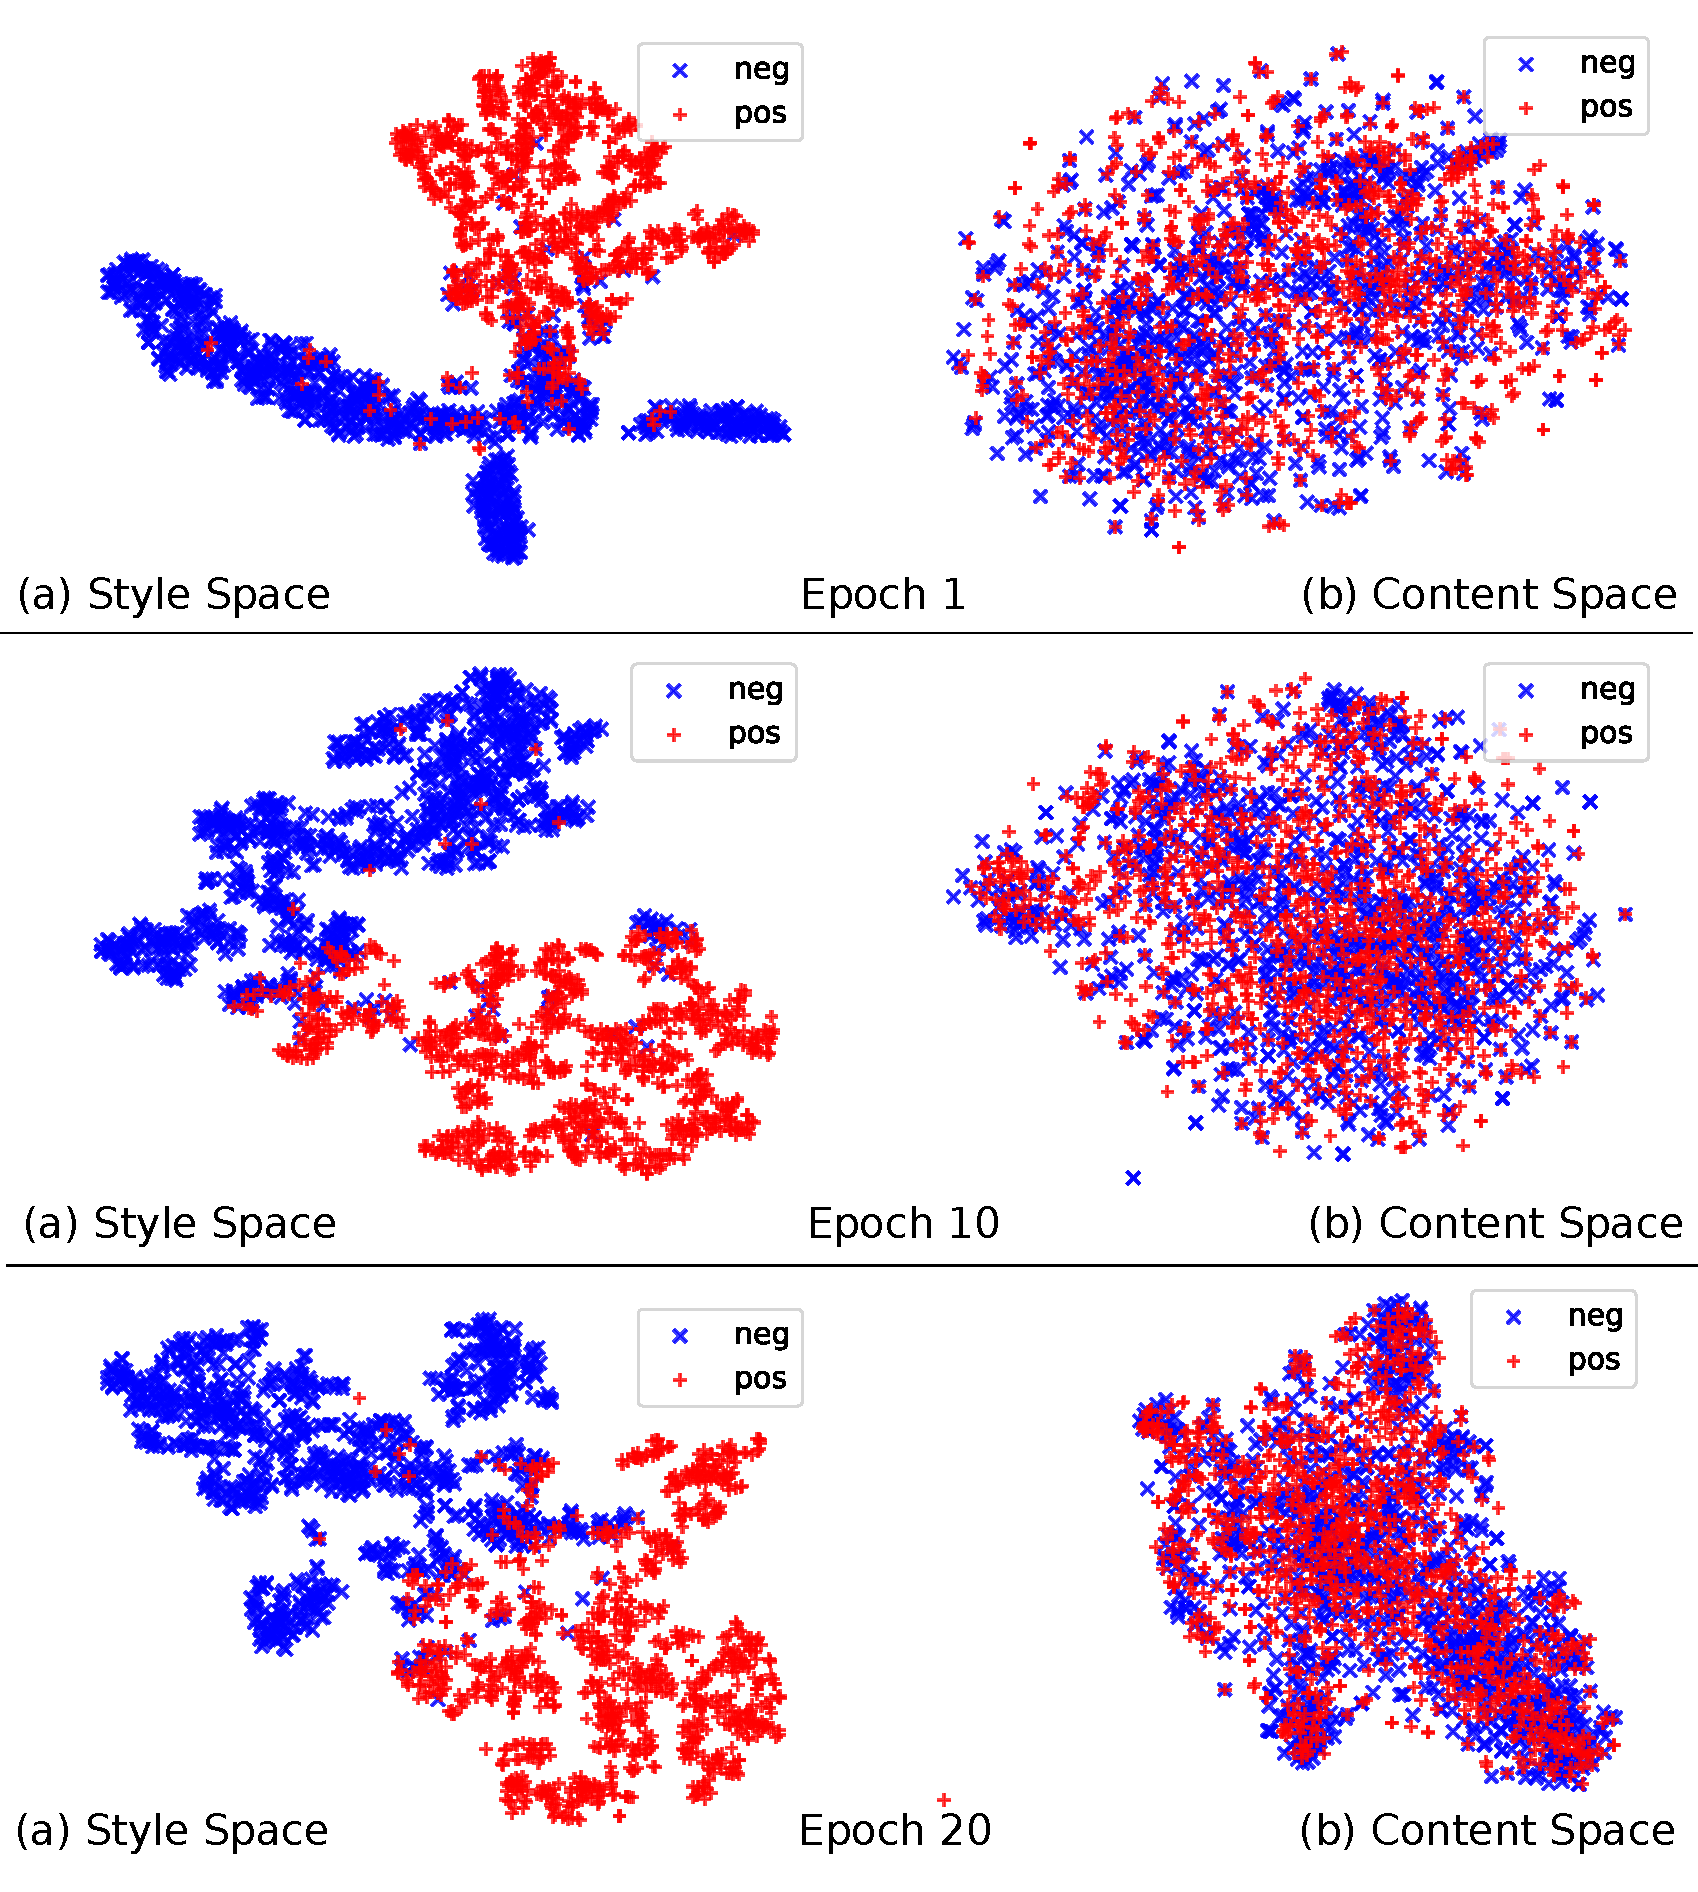
\includegraphics[width=\linewidth]{latent-spaces-dae}
	\caption{T-SNE Plots: (a) Style and (b) Content Spaces - DAE Model}
	\label{fig:dae-tsne}
\end{figure}

\begin{figure}[ht]
	\captionsetup{justification=centering}
	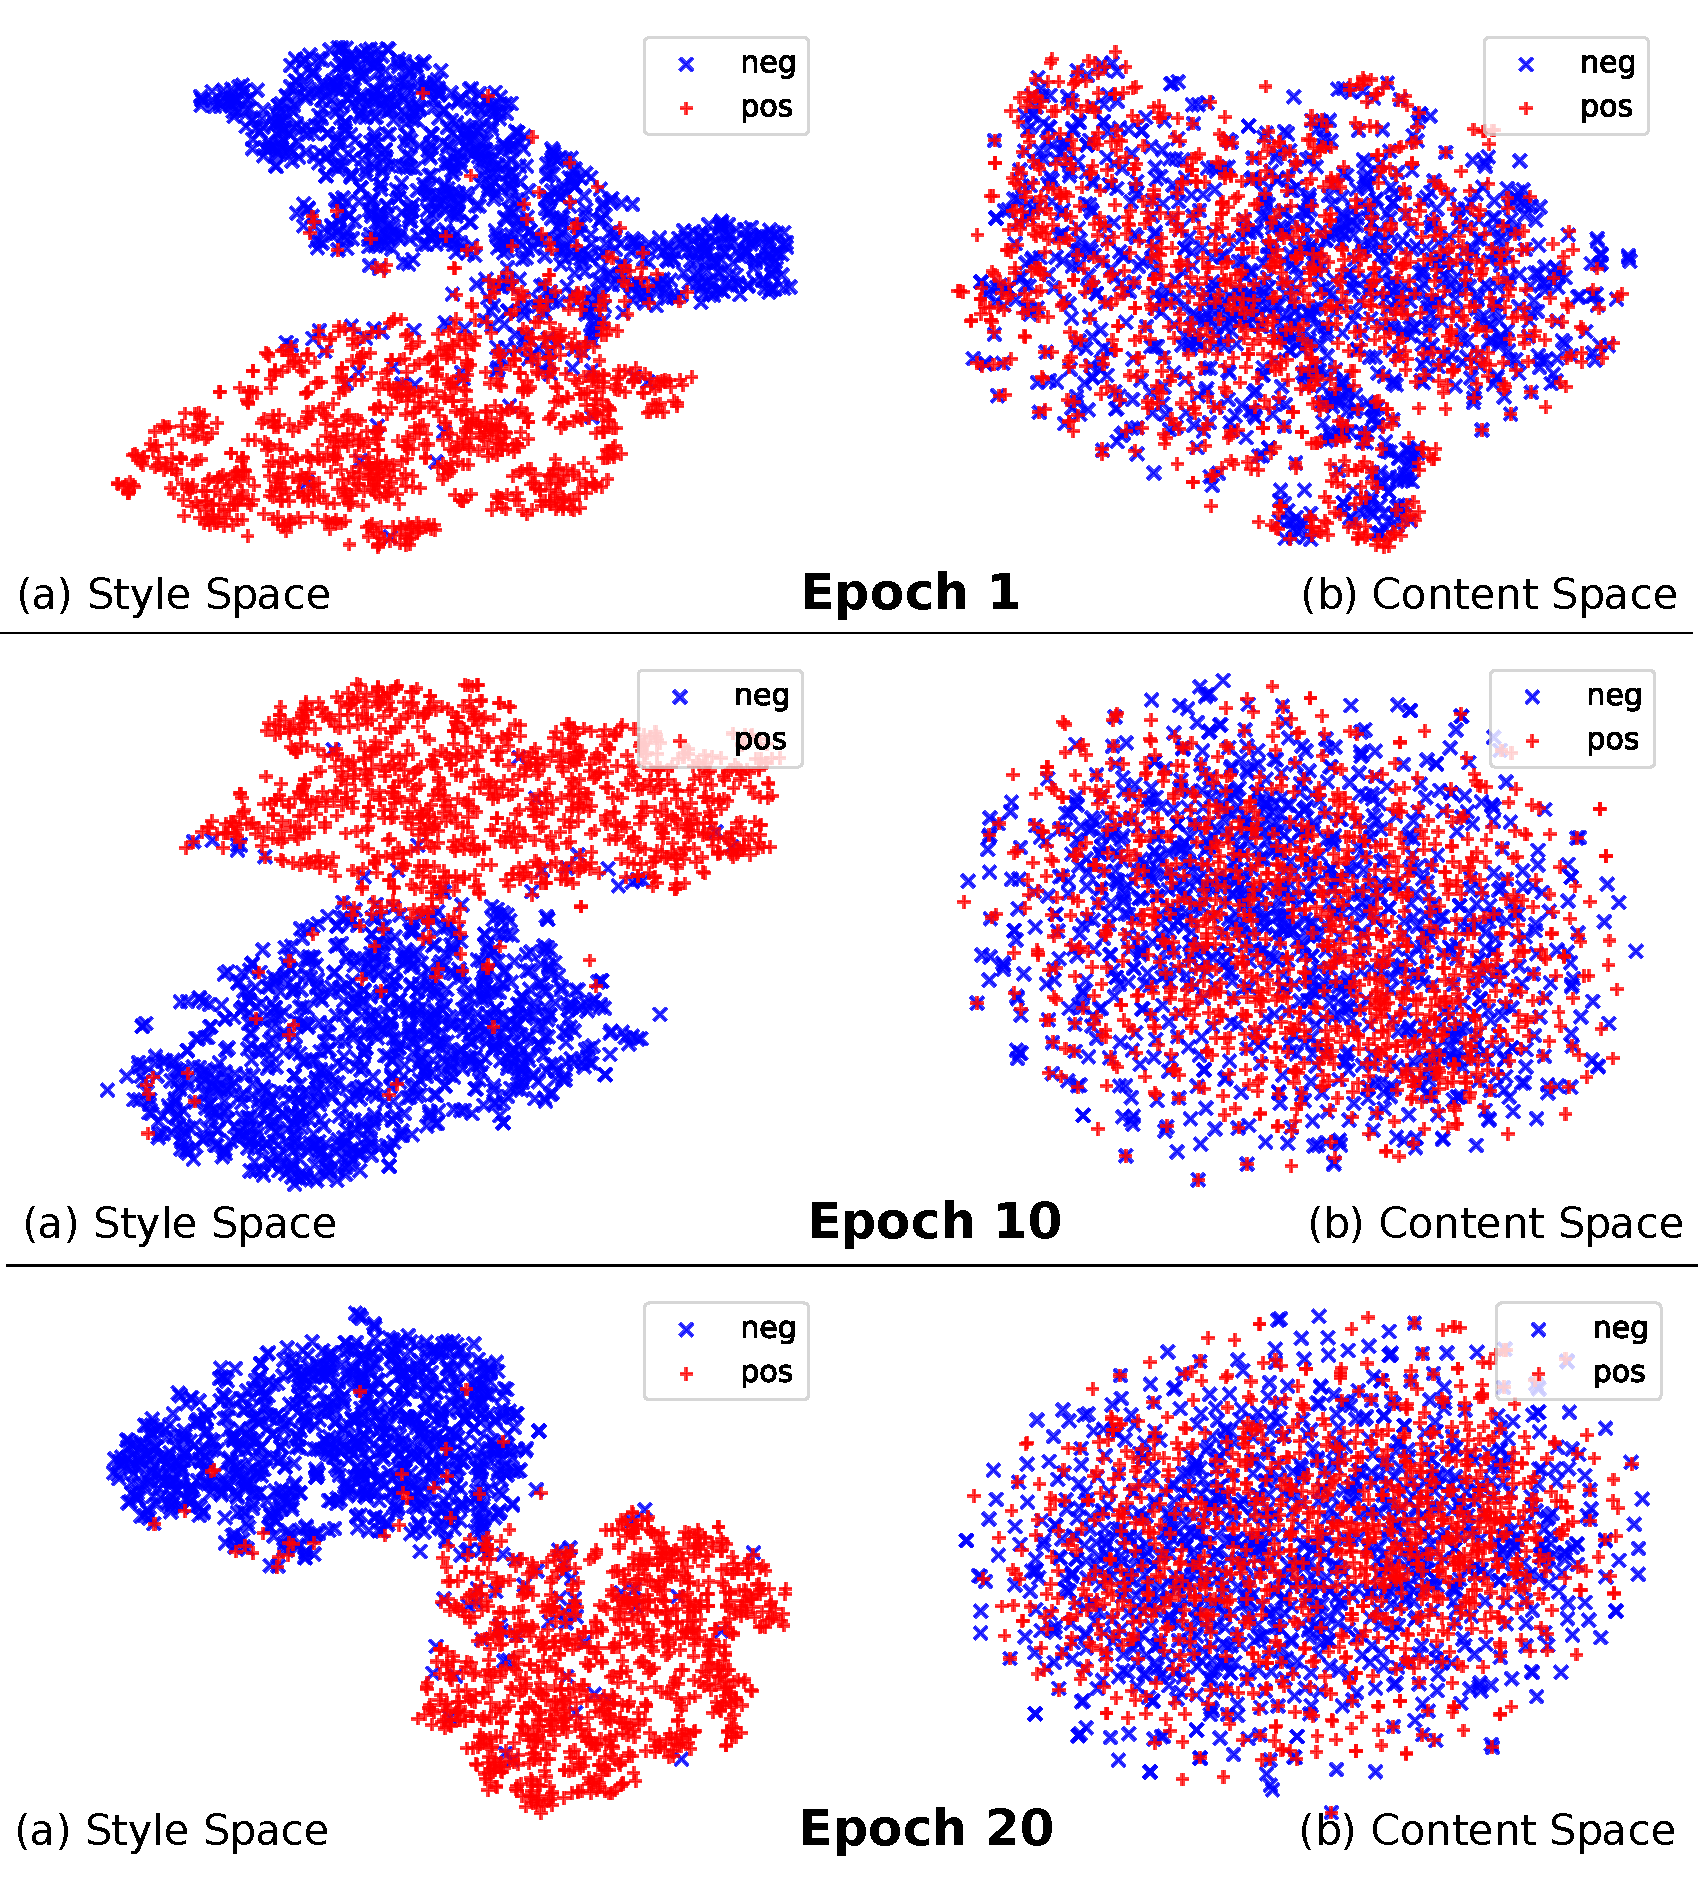
\includegraphics[width=\linewidth]{latent-spaces-vae}
	\caption{T-SNE Plots: (a) Style and (b) Content Spaces - VAE Model}
	\label{fig:vae-tsne}
\end{figure}


\subsection{Autoencoder} \label{ssec:seq2seq-autoencoder}

An autoencoder encodes an input to a latent vector space, which is usually of a much lower dimensionality than the input data, from which it decodes the input itself. By doing so, the autoencoder learns meaningful and compact representations of data. This serves as our primary learning objective. Besides, we also use the autoencoder for text generation in the style-transfer application.

Let $\rmx=(x_1, x_2, \cdots x_n)$ be an input sentence. The encoder encodes $\rm x$ by a recurrent neural network (RNN) with gated recurrent units (GRU) \cite{cho2014learning}, and obtains a hidden state $\bm h$.

Then a decoder RNN generates a sentence, which ideally should be $\rmx$ itself. Suppose at a time step $t$, the decoder RNN predicts the word $x_t$ with probability $p(x_t|\bm h, x_1\cdots x_{t-1})$, then the autoencoder is trained with cross-entropy loss, given by
\begin{equation}
	\loss{rec}(\bm\theta_E,\bm\theta_D)= -\sum_{t=1}^n \log p(x_t|\bm h, x_1\cdots x_{t-1})
\end{equation}
where $\bm\theta_E$ and $\bm\theta_D$ are the parameters of the encoder and decoder, respectively.

\subsubsection{Variational Autoencoder}

In addition to the deterministic auto-encoding objective presented above, we also implement a variational autoencoder (VAE) \cite{kingma2013auto}. The variational sampling and KL divergence losses are applicable to both the style space $\bm s$ and the content space $\bm c$, separately. The weights applied to each KL divergence loss are tuned independently as model hyperparameters.

Equation \ref{eqn:vae-rec} shows the reconstruction objective that is minimized in the VAE variant of our model.

\begin{align} \label{eqn:vae-rec}
	\loss{rec}(\bm\theta_E, \bm\theta_D) = \nonumber
	 & - \mathbb{E}_{q_{E}(\bm s|\rmx) q_{E}(\bm c|\rmx)} [\log p(\rmx|\bm s, \bm c)] \nonumber \\
	 & + \lambda_{\text{skl}} KL(q_{E}(\bm s|\rmx)||p(z)) \nonumber                             \\
	 & + \lambda_{\text{ckl}} KL(q_{E}(\bm c|\rmx)||p(z))
\end{align}
where $\lambda_{\text{skl}}$ and $\lambda_{\text{ckl}}$ are the weights for each of the KL divergence terms.

The motivation for using a variational autoencoder variant to compare the base deterministic autoencoder model to, is the property of VAEs that enable them to learn smooth and continuous latent spaces, without many dead zones in the latent space that cannot be decoded from. \cite{bowman2016generating} show this empirically by using the latent space of a text variational autoencoder to interpolate and generate novel sentences from the latent spaces between two valid sentences from a corpus.


Since these objectives train the model to reconstruct $\rmx$, they are also called \textit{reconstruction loss}. Besides the above reconstruction loss, we design three auxiliary losses to disentangle the latent space $\bm h$. In particular, we hope that $\bm h$ can be separated into two spaces $\bm s$ and $\bm c$, representing style and content respectively, i.e., $\bm h = [\bm s ; \bm c]$, where $[\cdot;\cdot]$ denotes concatenation. This is accomplished by the below auxiliary losses.



\begin{table*}[ht]
	\centering
	\begin{tabular}{| l | r | r |}
		\hline
		                                        & \tabh{DAE}                  & \tabh{VAE} \\
		\hline \hline
		Random/Majority guess                   & \multicolumn{2}{c|}{0.6018}              \\ \hline \hline
		Content latent space  ($\bm c$)         & 0.6137                      & 0.6567     \\ \hline
		Style latent space ($\bm s$)            & 0.7927                      & 0.7911     \\ \hline
		Complete latent space ($[\bm s;\bm c]$) & 0.7918                      & 0.7918     \\
		\hline
	\end{tabular}
	\caption{Style classification accuracy.}
	\label{tab:classification}
\end{table*}

\subsection{Multi-Task Classification} \label{ssec:multitask-classification-objective}

Our first auxiliary loss ensures the style space does contain style information. We build a classifier on the style space $\bm s$ predicting the true style label $y$, which is a part of the training data.

This loss can be viewed as a \textit{multi-task} loss, which makes the neural network not only decode the sentence, but also predicts its sentiment. Similar multi-task losses are used in previous work for sequence-to-sequence learning \cite{luong2015multi}, sentence representation learning \cite{jernite2017discourse} and sentiment analysis \cite{balikas2017multitask}, among others.

In our application, we follow previous work \cite{hu2017toward,shen2017style,fu2017style} and treat the sentiment as the style of interest. We introduce a multi-label classifier
\begin{equation} \label{eqn:class-pred}
	p(y' | \bm s; \bm\theta_\text{mult}) = \sigma(\bm w_\text{mult}^\top \bm s + b_\text{mult})
\end{equation}
where $\bm\theta_\text{mult}=[\bm w_\text{mult}; b_\text{mult}]$ are the classifier's parameters for multi-task learning, and $y'$ is the true label distribution.

This is trained using a simple cross-entropy loss.
\begin{equation} \label{eqn:multi-task-loss}
	\loss{mult}(\bm\theta_{E};\bm\theta_\text{mult}) =
	- \mathbb{E} [\log p(y' | \bm s; \bm\theta_\text{mult})]
\end{equation}
where $\bm\theta_E$ are the encoder's parameters.


\begin{table*}[ht]
	\centering
	\begin{tabular}{| l | r | r | r | r |}
		\hline
		\tabc{2}{Model}                       & \tabh{Transfer} & \tabh{Content}      & \tabh{Word}    & \tabh{Language} \\
		                                      & \tabh{Strength} & \tabh{Preservation} & \tabh{Overlap} & \tabh{Fluency}  \\
		\hline
		\hline
		Cross-Alignment \citep{shen2017style} & 0.8087          & 0.8920              & 0.2087         & -23.3886        \\
		\hline
		Style Embedding \citep{fu2017style}   & 0.1819          & 0.9586              & 0.6661         & -16.1711        \\
		\hline
		Ours (DAE)                            & 0.8425          & 0.8924              & 0.2552         & -16.4808        \\
		\hline
		Ours (VAE)                            & 0.8903          & 0.8824              & 0.2105         & -14.4099        \\
		\hline
		Ours (WAE-IMQ)                        & 0.8262          & 0.8844              & 0.2219         & -15.2464        \\
		\hline
		Ours (WAE-RBF)                        & 0.8138          & 0.8848              & 0.2229         & -14.8628        \\
		\hline
	\end{tabular}
	\caption{Yelp Dataset - Comparison with previous approaches.}
	\label{tab:yelp-comparison-previous}
\end{table*}

\begin{table*}[ht]
	\centering
	\begin{tabular}{| l | r | r | r | r |}
		\hline
		\tabc{2}{Model}                       & \tabh{Transfer} & \tabh{Content}      & \tabh{Word}    & \tabh{Language} \\
		                                      & \tabh{Strength} & \tabh{Preservation} & \tabh{Overlap} & \tabh{Fluency}  \\
		\hline
		\hline
		Cross-Alignment \citep{shen2017style} & 0.6063          & 0.8933              & 0.0241         & -26.3093        \\
		\hline
		Style Embedding \citep{fu2017style}   & 0.4165          & 0.9332              & 0.3588         & -28.1346        \\
		\hline
		Ours (DAE)                            & 0.7032          & 0.9178              & 0.1305         & -32.4184        \\
		\hline
		Ours (VAE)                            & 0.7259          & 0.9090              & 0.0814         & -28.4953        \\
		 \hline
		 Ours (WAE-IMQ)                        & 0.6830          & 0.9125              & 0.1074         & -30.7064        \\
		 \hline
		 Ours (WAE-RBF)                        & 0.6895          & 0.9169              & 0.1272         & -32.1801        \\
		\hline
	\end{tabular}
	\caption{Amazon Dataset - Comparison with previous approaches.}
	\label{tab:amazon-comparison-previous}
\end{table*}


\subsection{Adversarial Style Discrimination} \label{ssec:adversarial-style-objective}

The above multi-task loss only operates on the style space, but does not have an effect on the content space $\bm c$.

We therefore apply an adversarial loss to disentangle the content space from style information, inspired by adversarial generation~\cite{goodfellow2014generative}, adversarial domain adaptation~\cite{liu2017adversarial}, and adversarial style transfer~\cite{fu2017style}.

The idea of adversarial loss is to introduce an objective that deliberately discriminates the true style label $y$ on the content vector $\bm c$. Then the autoencoder is trained to learn such a content vector space that its adversary cannot predict style information from it.

Concretely, the adversarial discriminator predicts style $y$ by computing a softmax distribution over the possible class labels
\begin{equation}
	p(y' | \bm c; \bm\theta_\text{dis}) = \sigma(\bm w_\text{dis}^\top \bm c + b_\text{dis})
\end{equation}
where $\bm\theta_\text{dis}=[\bm w_\text{dis}; b_\text{dis}]$ are the parameters of the adversary, and $y'$ is the true label distribution.

It is trained by minimizing the following objective, using a cross-entropy loss.
\begin{equation} \label{eqn:adv-disc-loss}
	\loss{dis}(\bm\theta_\text{dis}) =
	- \mathbb{E} [\log p(y' | \bm c; \bm\theta_\text{dis})]
\end{equation}
The adversarial loss appears similar to the multi-task loss as in Equation \ref{eqn:multi-task-loss}. However, it should be emphasized that, for the adversary, the gradient is not propagated back to the autoencoder, i.e. the variables in $\bm c$ are treated as shallow features.

Having trained an adversary, we would like the autoencoder to be tuned in such an \textit{ad hoc} fashion, that $\bm c$ is not discriminative in style. In other words, we penalize the Shannon entropy of the adversary's prediction, given by
\begin{equation}
	\loss{adv}(\bm\theta_E)=\mathcal{H}(p_\text{dis}(y|\bm c))
\end{equation}
where $\mathcal{H}=-\sum_{i\in\text{labels}}p_i\log p_i$ is the entropy and $y$ is the predicted distribution over the style labels. The adversarial objective is maximized, in this phase, with respect to the encoder.

\begin{table*}[ht]
	\centering
	\begin{tabular}{| l | r | r | r | r |}
		\hline
		\tabc{2}{Objectives}                                     & \tabh{Transfer} & \tabh{Content}      & \tabh{Word}     & \tabh{Language}   \\
		                                                         & \tabh{Strength} & \tabh{Preservation} & \tabh{Overlap}  & \tabh{Fluency}    \\
		\hline
		\hline
		$\loss{rec}$                                             & 0.1436          & \textbf{0.9154}     & \textbf{0.3288} & -14.2781          \\
		\hline
		$\loss{rec}$, $\loss{adv}$                               & 0.7274          & 0.8800              & 0.2037          & -14.1567          \\
		\hline
		$\loss{rec}$, $\loss{mult}$                              & 0.7894          & 0.8976              & 0.2589          & -14.5607          \\
		\hline
		$\loss{rec}$, $\loss{badv}$                              & 0.1677          & 0.9147              & 0.3282          & -14.4486          \\
		\hline
		$\loss{rec}$, $\loss{adv}$, $\loss{mult}$                & \textbf{0.8903} & 0.8824              & 0.2105          & -14.4099          \\
		\hline
		$\loss{rec}$, $\loss{adv}$, $\loss{badv}$                & 0.7491          & 0.8827              & 0.2022          & -14.3568          \\
		\hline
		$\loss{rec}$, $\loss{mult}$, $\loss{badv}$               & 0.7832          & 0.8958              & 0.2567          & -14.3373          \\
		\hline
		$\loss{rec}$, $\loss{adv}$, $\loss{mult}$, $\loss{badv}$ & 0.8846          & 0.8782              & 0.1970          & \textbf{-14.0479} \\
		\hline
	\end{tabular}
	\caption{Ablation test.}
	\label{tab:ablation-results}
\end{table*}

\subsection{Adversarial Bag-of-Words Discriminator} \label{sec:adversarial-bow-objective}

In addition to the auxiliary losses used above, we also propose a novel bag-of-words discriminator on the style space. The motivation for having this objective is to try and emulate the adversarial signal provided by the style discriminator, and do the same for the content. Here, we define the content of the sentence as the words from the original sentence without any words that are discriminative of style. The input sentences $\rmx$ are represented as vectors of the same size as the corpus vocabulary, with each index of the vector a discrete probability of a word's presence in the sentence. Therefore, this bag-of-words representation is comprised of only 0s and 1s.

The bag-of-words discriminator uses the style vector $\bm s$ produced by the autoencoder model and tries to predict the true bag-of-words distribution using a set of parameters that are distinct from those of the autoencoder. The discriminator uses a logistic regression to predict a probability of each word's occurrence in the original sentence, between 0 and 1.
\begin{equation}
	p(b' | \bm s; \bm\theta_\text{bow}) = \sigma(\bm w_\text{bow}^\top \bm s + b_\text{bow})
\end{equation}
where $\bm\theta_\text{bow}=[\bm w_\text{bow}; b_\text{bow}]$ are the classifier's parameters for bag-of-words prediction, and $b'$ is the true word distribution.

This objective is trained in a similar method to the style adversary, using a cross-entropy loss
\begin{equation} \label{eqn:adv-bow-disc-loss}
	\loss{bow}(\bm\theta_\text{bow}) =
	- \mathbb{E} [\log p(b' | \bm c; \bm\theta_\text{bow})]
\end{equation}
We also refrain from propagating the effects of this discriminator loss $\loss{bow}$ to the encoder parameters, ensuring that the parameters that each adversary and the autoencoder can update are mutually exclusive.

Similar to the style adversary, the empirical Shannon entropy of the predicted distribution is provided as a training signal for the autoencoder model to maximize.
\begin{equation}
	\loss{badv}(\bm\theta_E) = \mathcal{H}(p_\text{bow}(b | \bm s))
\end{equation}
where $b$ is the predicted word distribution.

The motivation for this adversarial loss is similar to the one used in the context of the style discriminator. We want to encourage the encoder to learn a representation of style $\bm s$ that the bag-of-words discriminator cannot predict most of the original words from.

\subsection{Training Process}

The overall loss $\loss{ovr}$, used for the autoencoder, is thus comprised of four different objectives: the reconstruction objective, the multi-task objective and the style and content adversaries.
\begin{align*}
	\loss{ovr} =
	 & \loss{rec}(\bm\theta_E, \bm\theta_D) - \lambda_\text{adv} \loss{adv}(\theta_E) +                                \\
	 & \lambda_\text{mult} \loss{mult} (\bm\theta_E,\bm\theta_\text{mult}) - \lambda_\text{badv} \loss{badv}(\theta_E)
\end{align*}
where $\lambda_\text{mult}$, $\lambda_\text{adv}$ and $\lambda_\text{badv}$ balance the model's auxiliary losses.

To put it all together, our training process is a loop of the following processes:
\begin{algorithm}[ht]
	\While{epochs remaining}{
		minimize $\loss{dis}(\bm\theta_\text{dis})$ w.r.t. $\bm\theta_\text{dis}$\;
		minimize $\loss{bow}(\bm\theta_\text{bow})$ w.r.t. $\bm\theta_\text{bow}$\;
		minimize $\loss{ovr}$ w.r.t. $\bm\theta_E, \bm\theta_D, \bm\theta_\text{mult}$\;
	}
\end{algorithm}

We use the Adam optimizer \cite{kingma2014adam} with an initial learning rate of $10^{-3}$ and train the model for 20 epochs. Both the autoencoder and its adversary are trained once per epoch with $\lambda_\text{mult} = 1$, $\lambda_\text{adv} = 0.3$ and $\lambda_\text{bow} = 0.001$. For the VAE model, we set $\lambda_{\text{skl}} = 0.03$ and $\lambda_{\text{ckl}} = 0.03$.

\subsection{Generating Style-Transferred Sentences} \label{ssec:sentence-generation}

A direct application of our disentangled latent space is style transfer for natural language generation. For example, we can generate a sentence with generally the same meaning (content) but an opposite sentiment.

Let $\rmx^*$ be an input sentence with $\bm s^*$ and $\bm c^*$ being the encoded, disentangled style and content vectors, respectively. If we would like to transfer its content to a different style, we compute an empirical estimate of the target style's vector $\hat{\bm s}$ by
\begin{equation*}
	\hat{\bm s}=\frac{\sum_{i\in\text{target style}}\bm s_i}{\text{\# target style samples}}
\end{equation*}
The inferred target style $\hat{\bm s}$ is concatenated with the encoded content $\bm c^*$ for decoding (Figure~\ref{fig:model-inference-overview}).

\begin{table*}[ht]
	\centering
	\begin{tabular}{| p{0.3\linewidth} | p{0.3\linewidth} | p{0.3\linewidth} |}
		\hline
		\tabc{2}{Original (Positive)}                          & \tabh{DAE Transferred}                                         & \tabh{VAE Transferred}                                      \\
		                                                       & \tabh{(Negative)}                                              & \tabh{(Negative)}                                           \\
		\hline
		\hline
		i would recommend a visit here                         & i would not recommend this place again                         & i would not recommend this place for my experience          \\
		\hline
		the restaurant itself is romantic and quiet            & the restaurant itself is soooo quiet                           & the restaurant itself was dirty                             \\
		\hline
		my experience was brief but very good                  & my experience was very loud and very expensive                 & my experience was ok but not very much                      \\
		\hline
		the food is excellent and the service is exceptional   & the food is by the worst part is the horrible costumer service & the food was bland and i am not thrilled with this          \\
		\hline
		the food is very very amazing like beef and fish       & the food is very horrible i have ever had mostly fish          & the food is very bland and just not fresh                   \\
		\hline
		we will definitely come back here                      & we will not come back here again                               & we will never come back here                                \\
		\hline
		both were very good                                    & everything was very bland                                      & both were very bad                                          \\
		\hline
		\hline
		\hline
		\tabc{2}{Original (Negative)}                          & \tabh{DAE Transferred}                                         & \tabh{VAE Transferred}                                      \\
		                                                       & \tabh{(Positive)}                                              & \tabh{(Positive)}                                           \\
		\hline
		\hline
		so nasty                                               & so helpful                                                     & so fabulous                                                 \\
		\hline
		consistently slow                                      & consistently awesome                                           & fast service                                                \\
		\hline
		crap fries hard hamburger buns burger tasted like crap & cheap and yummy sandwiches really something different          & yummy hamburgers and blue cheese bagels are classic italian \\
		\hline
		oh and terrible tea                                    & oh and awesome tea                                             & oh and great tea                                            \\
		\hline
		the interior is old and generally falling apart        & the interior is clean and orderly as entertaining              & the interior is old and noble                               \\
		\hline
		front office customer service does not exist here      & front office is very professional does you                     & kudos to customer service is very professional              \\
		\hline
		the crust was kinda gooey like                         & the crust is kinda traditional                                 & the crust is soooooo worth it                               \\
		\hline
	\end{tabular}
	\caption{Examples of style-transfer generation.}
	\label{tab:transfer-samples}
\end{table*}

\section{Experiments}

\subsection{Datasets}

We conduct experiments on two datasets, the details for which are given below. Both of these datasets evaluate the task of sentiment transfer.

\subsubsection{Yelp Service Reviews}

We use a Yelp review dataset \citep{challenge2013yelp}, which has been sourced from the code repository accompanying the implementation of the paper by \citet{shen2017style} open-sourced by the authors~\footnote{\url{https://github.com/shentianxiao/language-style-transfer}}. It contains 444101, 126670 and 63483 sentences for train, validation, and test, respectively, each sampling accompanied by binary sentiment labels. The maximum sentence length is 15, and the vocabulary size is about 9200.

\subsubsection{Amazon Product Reviews}

We also use an Amazon product reviews dataset~\footnote{\url{http://jmcauley.ucsd.edu/data/amazon/}}, following \citet{fu2017style}. The reviews were sourced from the code repository accompanying the paper~\footnote{\url{https://github.com/fuzhenxin/text_style_transfer}}. It contains 559142, 2000, 2000 sentences for train, validation, and test, respectively, each sampling accompanied by binary sentiment labels. The maximum sentence length is 20, and the vocabulary size is about 58000.

\subsection{Evaluation Metrics}

We evaluate our method using four metrics: style transfer strength, content preservation, word overlap, and language fluency

\subsubsection{Style Transfer}
We train a CNN style classifier \cite{kim2014convolutional} and predict the accuracy of the generated sentences. While the style classifier itself may not be perfect, it provides a quantitative way of evaluating the strength of style transfer \cite{hu2017toward,shen2017style,fu2017style}.

\subsubsection{Content Preservation}
We compute a sentence embedding by min, max, and average pooling of word embeddings; then a cosine similarity is computed to evaluate how close two sentences are in meaning. Here, sentiment words from a stop list \cite{hu2004mining} are removed \cite{fu2017style}.

\subsubsection{Word Overlap}
We also utilize a simpler unigram overlap metric. Given a source sentence $x$ and an attribute style transferred sentence $y$, let $w_x$ and $w_y$ be the set of unique words present in $x$ and $y$ respectively. Then, the word overlap score can be calculated using $$\text{word-overlap} = \frac{count(w_x \cap w_y)}{count(w_x \cup w_y)}$$ which is simply a normalized measure of overlapping unigrams in the source and target.

\subsubsection{Language Fluency}
We use a trigram based Kneser–Ney Smoothed language model \citep{kneser1995improved} as a quantifiable and automated scoring metric by which to assess the quality of generated sentences. It calculates the probability distribution of trigrams in a document based on their occurrence statistics, to build a language model. We train this language model model on the complete corpus that we evaluate our style transfer models with. The log-likelihood scores, as predicted by the Kneser-Ney language model, and aggregated over the generated corpus, is reported as the indicator for language fluency.


\section{Discussion}

\subsection{Disentangling Latent Space}

We first analyze how the style (sentiment) and content of the latent space are disentangled. We train a classifiers on the different latent spaces, and show results in Table~\ref{tab:classification}. These are results from the experiments on the Yelp Dataset.

We see that the 128-dimensional content vector $\bm c$ is not particularly discriminative for style. It achieves accuracies that are only slightly better than random/majority guess. However, the 8-dimensional style vector $\bm s$, despite its low dimensionality, achieves significantly higher style classification accuracy. When combining content and style vectors, we achieve no further improvement. These results verify the effectiveness of our disentangling approach, because the style space does contain style information, whereas the content space doesn't.

We show t-SNE plots of both the deterministic autoencoder (DAE) and the variational autoencoder (VAE) models in Figure \ref{fig:dae-tsne} and Figure \ref{fig:vae-tsne}, respectively.


As can be seen from the t-SNE plots, sentences with different styles are noticeably separated in a cleaner manner in the style space (LHS), but are indistinguishable in the content space (RHS). It is also evident that the latent space learned by the variational autoencoder is significantly smoother and continuous than the one learned by the deterministic autoencoder.


\subsection{Style-Transfer Sentence Generation}

We apply the disentangled latent space to a style-transfer sentence generation task, where the goal is to generate a sentence with different sentiment (style).

We compare our approach with state-of-the-art previous work in Table~\ref{tab:yelp-comparison-previous} and Table~\ref{tab:amazon-comparison-previous}. We re-conducted the experiments with their publicly available code and data.
Results show that, our approach achieves a comparable content-preservation and word overlap scores to previous work, but significantly better style-transfer scores, showing that our disentangled latent space can be used for better style-transfer sentence generation. Our VAE model is also the most fluent for the Yelp dataset task.

Table~\ref{tab:ablation-results} presents the results of an ablation test. We see that both the style adversarial loss and multi-task classification loss play a role in the strength of style transfer, and that they can be combined to further improve performance. Also, the combination of all the losses described yields the best language fluency score.

Some examples of style-transfer sentence generation are illustrated in Table~\ref{tab:transfer-samples}. We see that, with the empirically estimated style vector, we can flexibly control the sentiment of generated sentences.


\section{Conclusion and Future Work}
In this paper, we propose a simple yet effective approach for disentangling the latent space of neural networks by multi-task loss and adversarial loss. Our disentangled space can be applied to style-transfer sentence generation, achieving similar content- preservation scores but significantly higher style transfer strength compared to previous state-of-the-art work.

\bibliography{emnlp2018}
\bibliographystyle{acl-natbib}

\end{document}
